\documentclass{report}
\usepackage[utf8]{inputenc}
\usepackage{graphicx}
\usepackage{placeins}
\usepackage[official]{eurosym}
\usepackage[a4paper,left=1.5in,right=1.5in,top=1in,bottom=1in]{geometry}
\usepackage{subcaption}
\usepackage{array}
\usepackage{longtable}
\usepackage[usenames,dvipsnames]{color}
\usepackage[caption = false]{subfig}
\usepackage{amsmath}
\usepackage[export]{adjustbox}% http://ctan.org/pkg/adjustbox
\usepackage{listings}
\usepackage{titlesec}
\usepackage{fancyhdr}
\usepackage[titletoc]{appendix}

\newcolumntype{P}[1]{>{\raggedright\arraybackslash}p{#1}}

 \lstset{ 
  numberblanklines=true,
  language=R,                     % the language of the code
  basicstyle=\small\ttfamily, % the size of the fonts that are used for the code
  numbers=left,                   % where to put the line-numbers
  numberstyle=\small\color{Blue},  % the style that is used for the line-numbers
  stepnumber=1,                   % the step between two line-numbers. If it is 1, each line
                                  % will be numbered
  numbersep=5pt,                  % how far the line-numbers are from the code
  backgroundcolor=\color{white},  % choose the background color. You must add \usepackage{color}
  showspaces=false,               % show spaces adding particular underscores
  showstringspaces=false,         % underline spaces within strings
  showtabs=false,                 % show tabs within strings adding particular underscores
  frame=false,                   % adds a frame around the code
  rulecolor=\color{black},        % if not set, the frame-color may be changed on line-breaks within not-black text (e.g. commens (green here))
  tabsize=2,                      % sets default tabsize to 2 spaces
  captionpos=b,                   % sets the caption-position to bottom
  breaklines=true,                % sets automatic line breaking
  breakatwhitespace=false,        % sets if automatic breaks should only happen at whitespace
  keywordstyle=\color{RoyalBlue},      % keyword style
  commentstyle=\color{YellowGreen},   % comment style
  stringstyle=\color{ForestGreen}      % string literal style
} 

% package for indent width
\usepackage[neverdecrease]{paralist}
\usepackage{setspace}
% set indent width for first and second itemize/enumerate
\setdefaultleftmargin{0.6cm}{0.5cm}{}{}{}{}
\newcommand\tab[1][1cm]{\hspace*{#1}}

% correct bad hyphenation here
\hyphenation{op-tical net-works semi-conduc-tor neighbors}

% Disable first word indent.
\setlength{\parindent}{0pt}

\DeclareMathOperator*{\argmax}{argmax}

\renewcommand{\baselinestretch}{1.1} 

\usepackage[colorinlistoftodos]{todonotes}



\begin{document}
\title{Online Automated Multivariate Web Design Optimization}
\begin{titlepage}
	
	\newcommand{\HRule}{\rule{\linewidth}{0.5mm}} % Defines a new command for the horizontal lines, change thickness here
	
	\center % Center everything on the page
	 
	%----------------------------------------------------------------------------------------
	%   HEADING SECTIONS
	%----------------------------------------------------------------------------------------
	
	\textsc{\LARGE VU University Amsterdam}\\[1.5cm] % Name of your university/college
	%----------------------------------------------------------------------------------------
	%   LOGO SECTION
	%----------------------------------------------------------------------------------------
	
	
\includegraphics{imgs/vu.png}\\[1cm] % Include a department/university logo - this will require the graphicx package
	 
	%----------------------------------------------------------------------------------------
	\textsc{\Large Computer Science}\\[0.5cm] % Major heading such as course name
	\textsc{\large Internet and Web Technology}\\[1.0cm] % Minor heading such as course title
	\textsc{\Large  \bfseries Master Thesis}\\[0.5cm]
	
	%----------------------------------------------------------------------------------------
	%   TITLE SECTION
	%----------------------------------------------------------------------------------------
	
	\HRule \\[0.4cm]
	{ \huge Online Automated Multivariate Web Design Optimization}\\[0.1cm] % Title of your document
	\HRule \\[2.5cm]
	 
	%----------------------------------------------------------------------------------------
	%   AUTHOR SECTION
	%----------------------------------------------------------------------------------------
	
	\begin{minipage}{0.4\textwidth}
		\begin{flushleft} \large
			\emph{Author:}\\
			Laurens \textsc{Verspeek} % Your name
		\end{flushleft}
	\end{minipage}
	~
	\begin{minipage}{0.4\textwidth}
		\begin{flushright} \large
			\emph{Supervisor:} \\
			Ana \textsc{Oprescu} % Supervisor's Name
		\end{flushright}
	\end{minipage}\\[2cm]
	
	% If you don't want a supervisor, uncomment the two lines below and remove the section above
	%\Large \emph{Author:}\\
	%John \textsc{Smith}\\[3cm] % Your name
	
	%----------------------------------------------------------------------------------------
	%   DATE SECTION
	%----------------------------------------------------------------------------------------
	
	{\large - 2016 -}\\[2cm] % Date, change the \today to a set date if you want to be precise
	
	
	
	\vfill % Fill the rest of the page with whitespace
	
\end{titlepage}
\thispagestyle{plain}
\pagestyle{fancy}
\fancyhf{}
\fancyhead[L]{\nouppercase{\leftmark}}
\fancyhead[R]{\thepage}

\begin{abstract}
Nowadays, there are over 1 billion websites online in the world wide web~\cite{numwebsites}. Modern web applications need to adapt to many different users. The user preferences are often hard to completely determine at design time. Therefore, these web applications are typically tested and refined at run-time to better determine the user preferences or to discover changed user preferences. These user-intensive websites increasingly rely on \textit{online-controlled experiments}~\cite{kohavi2007practical, kohavi2013online}, where different variants are being tested on live visitors. Technological advances in web design imply a large search space. A common strategy is sampling this huge search space. Current optimization strategies, such as A/B testing or multivariate testing, use \textit{manual} sampling, and are therefore time-consuming for the designer. The variants the designer samples from the large search space are static and cannot change during the test. After the test results are interpreted, the designer can setup new variants for the next static test. In this thesis we propose an online automated multivariate web design optimization system (AMOS) based on a genetic algorithm. This optimization technique will take away the manual part in website optimization by automating the sampling from the search space with a genetic algorithm. We will use a modified genetic algorithm, which uses fluid generations and keeps track of previous generations. By doing this we will get dynamic variants during the test and faster results. To validate the new optimization algorithm, it is implemented and tested on a live website with real users.
\end{abstract}
\setcounter{page}{3}

\newpage
\tableofcontents
\listoffigures
\listoftables
\newpage

\let\origchapter=\chapter
\let\origsection=\section

\renewcommand\chapter[1]{\origchapter{#1}\label{#1}}    
\renewcommand\section[1]{\origsection{#1}\label{#1}}

\chapter{Introduction}
Nowadays, there are over 1 billion websites online in the world wide web~\cite{numwebsites}. Modern web applications often have to deal and interact with many and evolving users. These applications that may need to handle thousands (or even millions) requests per day are called \textit{user-intensive applications}. User-intensive applications must satisfy the interaction requirements of many users, who often have different design preferences and different needs. These user preferences can also change and evolve over time. Designing a website that meets the different user preferences and is even able to evolve along with them is a key factor that can have huge implications on the success of the website~\cite{abtestwired}.\\

The  user preferences are often hard to completely determine at design time. 
Experts in the field of design can provide valuable insights to some degree about the user preferences that can be used to create an effective design for user-intensive applications. However, this information about the user preferences could be inaccurate or obsolete and may be too generic. It is impossible to prove if your design is the most optimal way, because there are no other data points to compare with. It is practically impossible to create a design for an application that is optimized for all user preferences up front. This can be proven by the fact that online controlled experiments, like A/B testing, have shown to be very successful. A few big examples are described later on in this section. Even if they were able to perfectly capture the user preferences when initially designing the application, the users, and with them the user preferences, evolve and change over time.\\

User-intensive web applications are typically tested and refined at run-time to better determine the user preferences or to discover changed user preferences. These user-intensive websites increasingly rely on \textit{online-controlled experiments\footnote{Also referred to as \textit{website optimization techniques} in this thesis}}~\cite{kohavi2007practical, kohavi2013online}, where different variants are being tested on live users. Technological advances in web design imply a large search space. Current optimization strategies, such as A/B testing or multivariate testing, use \textit{manual} sampling, and are therefore time-consuming for the designer. The variants the designer samples from the large search space are static and cannot change during the test. After the test results are interpreted, the designer can setup new variants for the next static test.\\

Many online companies use online controlled experiments to evaluate and optimize their applications. A few examples are Amazon~\cite{amazon}, eBay~\cite{ebay}, Facebook~\cite{facebook}, Google~\cite{google}, Groupon~\cite{groupon}, LinkedIn~\cite{linkedin}, Microsoft~\cite{microsoft}, Netflix~\cite{netflix} and many more big companies. Currently, the most widespread online controlled experiment approach used by companies is A/B testing~\cite{kohavi2013online}.\\

A/B testing is a technique where two different variants of an application are evaluated and compared to each other. The evaluation of the two variants is being done at run-time with live visitors. The two variants will be evenly split among the visitors. The evaluation is done by collecting data about some action of the visitors (like clicking a button, buying a product or signing up for a newsletter). The two different variants are compared based on this collected data. If one variant is significantly better than the other, that variant is selected and the other is disregarded. Designers often perform multiple A/B tests to gradually refine their application to meet the user preferences.\\

A/B testing is increasingly being used by many companies to evaluate and refine their their web applications~\cite{kohavi2013online}. In many cases A/B testing proved to be an effective evaluation and optimization tool~\cite{abtestwired, kohavi2007practical}. However, A/B testing suffers from several limitations. Running and interpreting an A/B test is a difficult and error prone activity~\cite{crook2009seven}. The selection of the variants for each A/B test is still a manual task that can be very time consuming.\\

Multivariate testing is another more advanced online controlled experiment technique where multiple variants can be tested at the same time. This is an improvement compared to the limitation of only two variants in A/B testing, but again is still limited to a static number of variants that the designer has to select manually per test. It is also more difficult to execute and interpret the statistics than A/B testing~\cite{diff}. In Section~\ref{Background and Problem Statement} more details are provided about the current state-of-the-art techniques regarding website optimization.\\

\section{Research question}
In this thesis we try to tackle the issues with the currently used techniques for website optimization by proposing a genetic algorithm that can optimize design parts of a web-page automatically in an evolutionary manner. When a genetic algorithm will be applied to optimize web design, it can continually search for optimal design variants. It can also adapt to the needs of diverse user groups and varying user preferences for web design. We can also automate the sampling of variants from the search space with genetic algorithms. The genetic algorithm will also have more dynamic variants for each test and will sample these variants automatically from the search space. This might even lead to solutions that would otherwise not be considered using traditional design methods. Website optimization is a search problem with a huge multi-dimensional search space. Genetic algorithms have been proven to be very successful in other areas for problems with large search spaces. Therefore our research question is:\\

\textit{Can a genetic algorithm automate and improve the real-world optimization process of web design?}\\

This thesis is organised as follows: Section~\ref{Background and Problem Statement} provides a detailed background on A/B testing and other testing techniques, and describes the problems of these techniques. Section~\ref{Related Work} reviews and discusses related work in the context of genetic algorithms. Section~\ref{AMOS: Automated Multivariate Optimization System} discusses our Automated Multivariate Optimization System (AMOS) and models the process of website optimization as a search problem. Section~\ref{System Architecture and Implementation} discusses the setup and implementation of AMOS in a framework that can be implemented easily on any (live) Web application. Section~\ref{Evaluation} evaluates the AMOS framework on real website with live users. Finally, Section~\ref{Conclusions} draws some conclusions and discusses future work.

\FloatBarrier
\chapter{Background and Problem Statement}
This section discusses in more detail how A/B testing and other online controlled experiment techniques work and states the existing limitations of these current testing techniques.
\section{A/B Testing} 
Currently, the most widespread online controlled experiment approach used by companies is A/B testing~\cite{kohavi2013online}. A/B testing is an online controlled experiment technique where two different variants of an application are evaluated and compared to each other. The evaluation of the two variants is being done at run-time with live visitors. The two variants will be evenly split among the visitors. The evaluation is done by measuring a certain business goal. In the context of web applications, this goal is almost exclusively \texit{conversion}. Conversion is the proportion of a website’s visitors taking a desired action, like clicking on a button, buying a product or signing up for a newsletter.\\

The two different variants are compared based on the conversion. Statistical analysis is used to do this comparison. If one variant is significantly better than the other, then that variant is selected and the other is discarded. Designers often perform multiple A/B tests to gradually refine their application to meet the user preferences. The overall process of A/B testing is exemplified in Figure~\ref{fig:abtesting}.\\

\begin{figure}[ht]
	\centering
	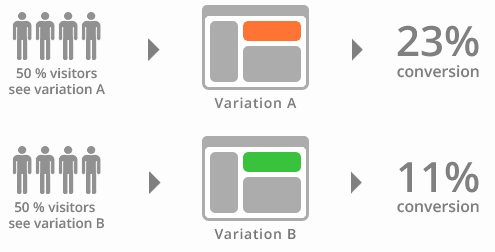
\includegraphics[width=\linewidth]{imgs/ab_testing.png}
	\caption{A/B Testing Process}
	\label{fig:abtesting}
\end{figure}
Figure~\ref{fig:abtesting} shows that half of the live users are randomly assigned to one of the two variants of the web applications that is being A/B tested: variant A (also called the control variant). This control variant is typically the current version of how the website looks. The other half of the visitors is assigned to variant B (also called the treatment variant). The treatment variant is usually a newer version of the web application whereof the designer thinks will perform better. The conversion for both variants is measured. If the difference is big enough and there are enough visitors, statistical analysis can prove that one variant is significantly better than the other variant. The best variant is retained and the other one is discarded. This statistical significance is commonly tested with a \emph{Two-sample hypothesis tests}, such as Student's t-tests or Welch's t-test~\cite{kohavi2007practical}.\\

Even though A/B testing is the most common website optimization tool in web industry~\cite{kohavi2007practical, kohavi2013online}, running and interpreting an A/B test is a difficult and error prone activity~\cite{crook2009seven}. The selection of the variants for each A/B test is still a manual task that can be very time consuming. A/B testing also suffers from several other limitations:

\begin{itemize}
	\item \textbf{Static number of variants.} While you may have many different variants you want to test on your website, A/B testing only allows for two variants per test run. After the test, new variants have to be manually created based on the previous test results. These variants can be used in the new test. Variants can not change during the test.
	\item \textbf{Selecting variants is a time-consuming manual activity}. For each new experiment the designer has to interpret the statistics of the results of the previous test and based on that interpretation, he has to provide the two variants to apply the next A/B test on. This is a time-consuming manual activity~\cite{crook2009seven}.
	\item \textbf{Quality of variants depends on quality of the designer} Quality of the variants (and therefore the quality of the test) for the next test depends on the domain knowledge of the designer and quality of the interpretation of the statistics of the previous test.
	\item \textbf{No optimal solution.} Even though a variant might be better than the original, you can never know if it is the best possible variant. Other variants might bring even bigger improvements.
	\item \textbf{Cannot take multiple different user preferences into account.} Different users might like different variants. Traditional A/B testing will pick only one variant for all users.
	\item \textbf{Cannot adapt to changing user preferences.} Even though variant A had better results than variant B a year ago, this does not mean that it will still perform better now.
	\item \textbf{Needs clear goals that can be measured by the computer}. In order to evaluate the different variants, you need clear goals to test on that are measurable (e.g. sales, user subscriptions, number of downloads etc.). Goals like improving brand reputation or supporting the company's public relations efforts can't be measured by user actions on the website.
	\item \textbf{Only measures quantity, not quality.} A/B testing measures conversions based on the occurrence of events, a binary value. Just because one version leads to more sign-ups or even sales does not mean that the other version has less value. The seemingly-successful variation may contain a change that specifically attracts the wrong kind of customers in larger numbers~\cite{abtestbad}. For example, by reducing the barriers to sign-up (e.g. by not requiring e-mail or full name), the number of sign-ups will probably increase, but there will also be a lot of fake accounts, therefore decreasing the average quality of customers.
\end{itemize}

The limitations mentioned above tend to be concrete obstacles for website optimization and they also make A/B testing an error-prone tool that may yield false and uncontemplated results.

\section{Multivariate Testing}
Multivariate testing is another approach that goes beyond the limitation of two variants. Multivariate testing allows to test multiple variants at the same time and see which one performs the best. This is obviously an improvement, but again is still limited to the developer/designer making a finite number of variants to test. The other limitations A/B testing has (stated in previous section) also apply for multivariate testing. The overall process of multivariate testing is exemplified in Figure~\ref{fig:mvtesting}.\\ 

\begin{figure}[ht]
	\centering
	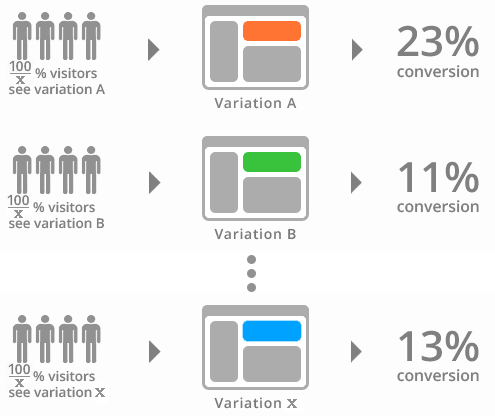
\includegraphics[width=\linewidth]{imgs/mv_testing.png}
	\caption{Multivariate Testing Process}
	\label{fig:mvtesting}
\end{figure}

Figure~\ref{fig:mvtesting} shows that in multivariate testing the visitors are divided between all the different variants of the website. This is much like in A/B testing, where the visitors are split between two variants of the website. Then the conversion rates of each variant are measured and compared to each other with statistical analysis (multivariate analysis).\\

Multivariate testing has some advantages and some disadvantages compared to A/B testing. For multivariate testing to give meaningful results, it needs a large sample of data~\cite{mvt}. This means that the web-page you are testing will need a lot of visitors in order to detect a significant difference between the different variants. Besides that multivariate testing requires high page traffic, it also requires more user input. The statistical analysis of a multivariate test is more complex than A/B testing, but it gives better insights of the performance of multiple elements of a website at the same time~\cite{kohavi2009controlled}. \\

The statistical analysis is typically done with analysis of variance (ANOVA)~\cite{iitsuka2015website}. ANOVA allows us to compare the different variants with each other and find significant differences in the conversion rates of the different variants. ANOVA is more efficient for multiple groups than a simple Students t-test, the test that is used in A/B testing. This means that if we want to test the same amount of variants as in one multivariate test, but instead we use multiple A/B tests, then we would need more visitors compared to A/B testing. However, when using multivariate testing more visitors are needed before any results can be provided compared to A/B testing. Overall, multivariate-testing is harder to execute and analyze and needs more visitors than A/B testing before it can provide any results.~\cite{diff, iitsuka2015website}.
\FloatBarrier

\chapter{Related Work}
In this section related state-of-the-art approaches that try to solve the website optimization problem with Genetic Algorithms are discussed. Three different approaches are discussed and their features are compared with each other in Table~\ref{tab:cfg}. The first column of that table shows the aim of our approach and states the features that we want our approach to have. More details about our approach will be explained in the next section.
\section{Theoretical Genetic Algorithm Framework}
The problem of optimizing and evolving web design of user-intensive applications at run-time is quite a new field and has not received much attention yet to the best of our knowledge. The first ones to introduce this problem Tamburrelli and Margara~\cite{tamburrelli2014towards}. They formalize A/B testing as a a Search-Based Software Engineering (SBSE) problem and they propose an initial prototype that relies on aspect-oriented programming and genetic algorithms. They use that prototype to demonstrate the practical feasibility of automated A/B testing through a set of synthetic experiments. The architecture of their setup can be found in Figure~\ref{fig:archpaper}.\\

\begin{figure}[ht]
	\centering
	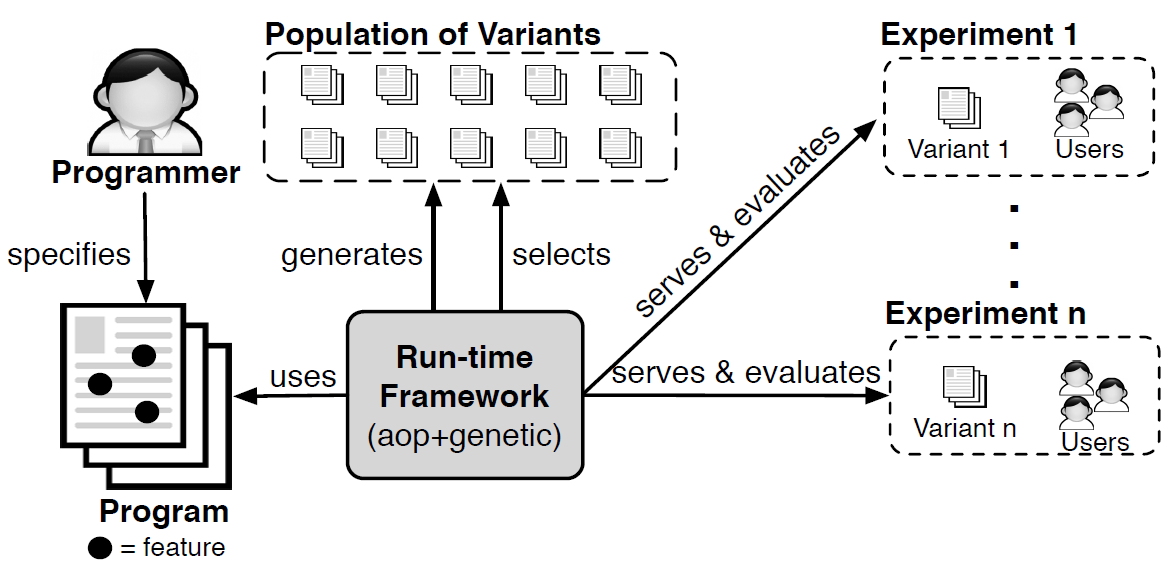
\includegraphics[width=\linewidth]{imgs/archpaper.PNG}
	\caption{Architecture for automated A/B testing as proposed by Tamburrelli and Margara~\cite{tamburrelli2014towards}.}
	\label{fig:archpaper}
\end{figure}

Although the use of genetic algorithms in this field is very interesting as also mentioned earlier in this thesis, this theoretical approach has several drawbacks as exemplified hereafter. First, the behaviour of their architecture still needs to be configured by specifying several parameters (e.g., the population size, selection strategy, and the termination condition). Experimental campaigns on real users will be required to further study and tune them appropriately. Second, they assume a-priori defined fitness values. The do this by assuming that there is one optimal value for each feature. Then they assume that these values are linearly correlated with the fitness value. This means that the closer you are to that optimal value, the better the fitness value. They also assume that the features are independent of each other. However, it is very unlikely that these assumptions will hold for real-world web applications. Features often have some sort of interaction effect between them. For example, users might like white text color, but not when that text is also on a white background color. Another unrealistic assumption they make is that each user can give a fitness value to each feature instantly. This is an unrealistic approach as in the real world you need many visitors to get a good reliable fitness value. They only tested their approach in a simulation, where they simulated 10 million users with the assumptions stated above.\\

\FloatBarrier
\section{Practical Genetic Algorithm Framework}
Genetify is a more concrete example of a project that tries to automate the process of A/B testing~\cite{genetify}. Genetify uses a genetic algorithm to optimize parts of a website. Developers define the different variants for each group of elements and they define the goals that are used as fitness function for the different variants. It does not use a true genetic algorithm as it for example did not allow for mutations. Also, the developer still has to create the different variants himself. One of the goals of this thesis is to also eliminate that manual work by creating the variants automatically (with certain set limitations). However, this project never saw a full release and at the time of writing this thesis the project was even discontinued. Greg Dingle, the creator of Genetify said that "the advertising market presented a much more lucrative opportunity"~\cite{genetifyquote}.\\

\section{Interactive Genetic Algorithms}
There is several related work~\cite{park2007webpage,oliver2002interactive,sorn2013web} that uses a specific type of implementation of genetic algorithms applied to web design creation. This technique is called Interactive Genetic Algorithm (IGA). IGA is a type of genetic algorithm where the evaluation part to retrieve a fitness value is done explicitly by the users~\cite{takagi2001interactive}. This is called human evaluation. This is very useful when it is difficult or even impossible to describe a computational fitness function. IGA will create the initial population with solutions and lets the users decide which (set of) solutions they prefer. These preferences are then used as a fitness function for the genetic algorithm.\\

The experiments of the various papers that implemented IGA~\cite{park2007webpage,oliver2002interactive,sorn2013web} show promising results when it comes to genetic algorithms in the field of web design. However, IGA can be very intrusive for people if performed on a production site, as they continually need to choose between different versions of designs. IGA can be useful in the process of creating a website design on a testing environment and using that information for the design on the final production site. However, with IGA the website design will stop evolving once you go live with your website, as you can't ask for user feedback anymore.\\

Therefore, we will not use IGA to solve the problem of evolving and refining applications after their deployment. Instead, we look for alternative, less intrusive ways to evaluate the 'fitness' of each individual variant.  This can be done by optimizing the business goals of a website. In most cases this goal is \textit{conversion}. Conversion is the proportion of a website’s visitors taking a desired action, like clicking on a button or buying a product. Conversion can be used as a fitness function for the genetic algorithm without any user interaction.\\

\begin{table}[h]
	
	\hskip-3.0cm
	\begin{tabular}{|p{3cm}|p{3.5cm}|p{3.5cm}|p{3.5cm}|p{3.5cm}|}
		\hline
		\textbf{Feature}                                  & \textbf{(Aim of) Our Approach} & \textbf{Genetify}                                   & \textbf{IGA approaches}                      & \textbf{Theoretical GA Framework} \\ \hline
		    
		Can be used for real-world websites               & Yes                            & Yes                                                 & Yes                                          & No                                \\ \hline
		Can be used for real-world \textbf{live} websites & Yes                            & Yes                                                 & No                                           & No                                \\ \hline
		Custom goals as fitness function                  & Yes                            & Yes                                                 & No (fitness is done by the users themselves) & No (unrealistic fitness function) \\ \hline
		Dynamic variants                                  & Yes                            & No                                                  & No                                           & No                                \\ \hline
		Calculations of statistical significance          & Yes                            & No                                                  & Yes                                          & No                                \\ \hline
		   
		"Unlimited" variants                              & Yes                            & No (designer still has to has to give the variants) & Yes                                          & Yes                               \\ \hline
		Mutation                                          & Yes                            & No                                                  & Yes                                          & Yes                               \\ \hline
		Automatic creation of variants                    & Yes                            & No                                                  & Yes                                          & Yes                               \\ \hline
		User profiles (multiple user preferences)         & Yes                            & No                                                  & No                                           & No                                \\ \hline
		
	\end{tabular}
	\caption {Comparison of features of the different website optimization techniques that are using a Genetic Algorithm}
	\label{tab:cfg}
\end{table}
\FloatBarrier

\chapter{AMOS: Automated Multivariate Optimization System}
Now that we looked at currently used techniques like A/B testing and multivariate testing and other related approaches concerning genetic algorithms, we will look at the goals of our approach. Our approach will try to solve the first six problems of A/B testing stated in Section~\ref{A/B Testing}. This means that we need to improve, but more importantly \textit{automate} the website optimization process to overcome the costly manual activity of the currently used website optimization techniques. The last two problems stated in the A/B testing section (\textit{Needs clear goals that can be measured by the computer} and \textit{Only measures quantity, not quality}) are not addressed in this thesis as we will focus on solving the other, in our eyes more important, problems first. Our approach will be an Automated Multivariate Optimization System (AMOS).\\

When we look at the drawbacks of the related techniques that already tried to solve these problems by using a Genetic Algorithm we first of all want a more realistic evaluation of the fitness values of the different variants. We want to automatically evaluate the variants. The evaluation of variants needs to be realistic and we therefore want to tackle the apriori fitness value assumption from the theoretical genetic algorithm framework, discussed in Section~\ref{Theoretical Genetic Algorithm Framework}. We will do this by replacing the unrealistic fitness function with a realistic fitness function based on conversion. As we also want to be able to test this on real-world live websites, we also need to tackle the simulation environment and thus reduce the number of visitors needed to be able to make a decision regarding which variants perform good.

\section{Online controlled experiments as a Search problem}
To be able to automatically solve the website optimization problem with genetic algorithms, we first need to rephrase it as an optimization problem. The terminology introduced in this section will be used in the remainder of this thesis. In order to rephrase online controlled experiments as an optimization problem, we will mostly adopt the conceptual foundations introduced in the paper \emph{Towards Automated A/B Testing}~\cite{tamburrelli2014towards} with some slight modifications and additions.\\

\begin{itemize}
	\item \textbf{Features.} From an abstract viewpoint a program $p$ can be viewed as a finite set of features: 
	      $$F_p = \{f_1...f_n\}$$
	\item \textbf{Domain.} Each feature $f_i$ has an associated domain $D_i$ that specifies which values are valid for $f_i$:
	      $$f_i \in D_i$$
	\item \textbf{Instantiation.}  An instantiation is a function  that associates a feature $f_i$ in $F_p$ with a specific value from its domain $D_i$.
	      $$I_{p,f_i} : f_i \rightarrow D_i$$
	      
	\item \textbf{Variants.} A concrete implementation of program $p$ is a variant $v$ of program $p$. To obtain a concrete implementation for a program $p$ it is necessary to specify the instantiations for all the features in $p$.
	      $$\forall f_i \in F_p, I_p(f_i)$$
	      
	\item \textbf{Constraints.} A \emph{normal constraint} $C_i$ is function that returns a subset of values in domain $D_i$ that are \emph{not} allowed for feature $f_i$.
	      $$ f_i \in (D_i - C(i))$$
	      A \emph{dependent constraint} is a function $C_{i,j} : D_i \rightarrow P(D_j)$ that, given a value $d_i \in D_i$ for a feature $f_i$, returns a subset of values in $D_j$ that are \emph{not} allowed for the feature $f_j$.
	      $$ f_j \in (D_j - C(i,j))$$
	\item \textbf{Assessment Function.} An assessment function is a function that associates to variant $v$ of a program a numeric value, which indicates the goodness of the variant with respect to the goal of the program. 
	      $$o(v) : v \rightarrow {\rm I\!R}$$ 
\end{itemize}

Given these premises, we can rephrase online controlled experiments as a search problem as follows.
Given a program $p$ characterised by a set of features $F_p$, a set of constraints
$C_p$, a set of (valid) variants $V_p$ and an assessment function $o(v)$, find the variant $\hat{v} \in V_p$ such that $\hat{v}$ maximizes $o(v)$:
$$\hat{v} = v \in V_p, \argmax\limits_v o(v)$$\\

\FloatBarrier
\section{Genetic Algorithm}
Genetic algorithm is an optimization method based on the process of natural selection. This heuristic is generally useful to generate good solutions to optimization problems. Techniques inspired by natural evolution are used, like \textit{selection, crossover} and \textit{mutation} to create new generations.~\cite{mitchell1998introduction} Selection means that the best evaluated chromosomes are moving on to the next generation. The genes of these chromosomes are also combined to create new chromosomes. This is called crossover. Mutation is some random change in one of the values of the individuals. Genetic algorithms use a fitness function to evaluate all the individuals in a population. Genetic Algorithms are useful for large search spaces, since the algorithm tries to find partial solutions to the optimization problem first and use the info of these solutions to pick better solutions from the large search space. They avoid the need to use brute-force methods, while still being able to explore a wide set of good solutions. Figure~\ref{fig:gaworkflow} shows the workflow of genetic algorithms.

\begin{figure}[ht]
	\centering
	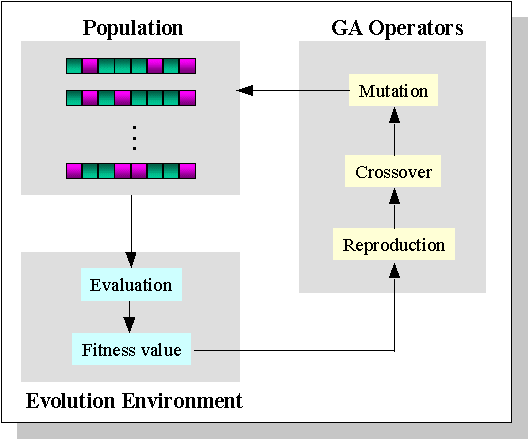
\includegraphics[width=0.7\linewidth]{imgs/gaworkflow.png}
	\caption{Workflow of a Genetic Algorithm}
	\label{fig:gaworkflow}
\end{figure}

The initial population is filled with completely random individuals from the search space. These individuals then get evaluated and based on the evaluation a new generation is created with the GA Operators.

As we do not want to mix the terms used for Genetic Algorithm with the terms used for website optimization, we will stick with the terms used in website optimization. Table~\ref{tab:map} shows the mapping from website optimization to Genetic Algorithm.
\FloatBarrier
\begin{table}[h]
	\centering
	\begin{tabular}{|l|l|}
		\hline
		\textbf{Website Optimization Problem} & \textbf{Genetic Algorithm} \\ \hline
		Variant                               & Chromosome                 \\ \hline
		Feauture                              & Gene                       \\ \hline
		Assessment function                   & Fitness function           \\ \hline
		Conversion                            & Fitness value              \\ \hline
		Test/Experiment                       & Generation                 \\ \hline
	\end{tabular}
	\caption{Mapping website optimization to Genetic Algorithm}
	\label{tab:map}
\end{table}
\FloatBarrier

By applying a genetic algorithm to web design optimization, the designer is not constrained to a static number of variants that need to be created manually. The genetic algorithm can automatically sample variants from the search space and produce a near-optimal variant after a period of testing. The genetic algorithm can also adapt the variants to new user preferences, as they can change over time.

\section{Hybridizing AMOS with Hill Climbing methods}
In order to speed up the process of website optimization, a combination of Genetic Algorithm and a \textit{Hill Climbing algorithm} is used. Hill Climbing uses only one solution at a time and  incrementally changes a single feature  of the solution.~\cite{russell2003artificial} If the new solution is better than the last solution, only then will that solution be used for new changes. If the new solution is worse than the previous one, it is discarded. Genetic Algorithms search multiple solutions at the same time, but when moving on to the next generation, it will only look at solutions from the current generation, even though older generations might have better solutions.\\ 

AMOS is a mix between these two types of optimization algorithms. We still have generations with multiple variants, like in Genetic Algorithms, but when creating a new generation, all the previous generations are taken into account instead of only the current generation.

\section{Statistical Significance}
In most fields where Genetic Algorithms are used, the fitness function can give a fitness value instantly and reliably to each variant in the population. However, in the field of website optimization we need to know the conversion of each variant in order to know which variants are performing best. Unfortunately, this is a metric that we can not determine instantly in a reliable fashion. Enough visitors per variant are needed to determine a good and reliable conversion rate for each variant.\\

Statistical analysis is used to calculate how many users we will need in order to detect reliable changes between the variants in a generation. When the differences between variants are significant, we know that we have enough visitors. Just as in multivariate testing, the statistical analysis will be performed with \textit{Analysis of Variance} (ANOVA).\\

ANOVA is a statistical method to compare the means of two or multiple groups. ANOVA can be used to do a statistical test to see whether the means of multiple groups are significantly different. It can therefore be seen as a generalization of the t-test for two groups, but applied to more than two independent groups.~\cite{gelman2005analysis}\\

The same result might be achieved by performing multiple two-sample t-test. However, when performing multiple t-tests or multiple pairwise comparisons after an ANOVA test, the chance of finding a incorrect significant difference between the means (rejecting the null hypothesis) increases. This is called the false positive error rate or Type I errors. For example, if a t-test is performed with a alpha level 0f 0.05, there is only a chance of 5\% of a false positive error. However, when 100 t-test are performed with alpha level 0.05, 5 out of those 100 t-test would incorrectly reject the null hypothesis. This means that the probability of at least one t-test with a false positive error is 99.4\% when the t-tests are independent. Techniques have been developed to control the false positive error rate associated with performing multiple statistical tests~\cite{westfall1993resampling}. Even though multiple two-sample t-test are conceptually similar to ANOVA, ANOVA results in less type I errors and is therefore less conservative.~\cite{miller2013analysis}\\

After performing an ANOVA, we may know that the conversion of one or multiple variants differs significantly from each other, but we do not know which pairs of variants differ significantly. At this point, we will conduct pairwise comparisons between the variant with the highest conversion and the variants with the lowest conversions.\\

The technique we used for our algorithm to control the Type I error for multiple pairwise comparisons is the \textit{Bonferroni correction}. It suggests that the p-value for each test must be equal to the original alpha divided by the number of tests. This correction is very conservative and can easily be replaced with less conservative correction techniques.\\

\section{Amount of visitors needed: sample size calculation}
By doing a power analysis, we can know in advantage how many visitors for each variant we will need to see a significant difference. Figure~\ref{fig:samplesize} shows the graph with the power analysis results. Figure~\ref{fig:samplesize2} is a zoomed in version of the tail of this graph for better readability. The graph can be used to see how many visitors are required to find a significant difference with 80\% certainty (Power = 0.8) in relation to the minimum increase in percentage you want to be able to detect for conversion. The Power value and the significance level are adopted as $\alpha = 0.05$ and $1 - \beta = 0.8$ from the study by Muller~\cite{muller1989statistical}. We will use these values throughout the remainder of this thesis. The graphs shows that if we want to detect small differences you will need more users per variant than when you want to detect big differences. The number of users needed is also dependent on the baseline conversion. The baseline conversion is the conversion where we compare to. In the graph we can see that we need more users to be able to detect differences for small baseline conversions than for larger baseline conversions. For example, we can see that if we have a baseline conversion of 3 percent and we to be able to detect a minimum increase of 100 percent, then we need about 450 users per variant.\\

The formula used to calculate the sample size given a certain power is from the book \textit{Sample Size Calculations in Clinical Research}~\cite{chow2007sample}. We use the parameter for the proportion of group A ($p_A$) as the baseline conversion. We stepwise increment the parameter for the proportion of group B ($p_B$) as a percentage increase of the baseline conversion. By calculating all the sample sizes ($n$) for these changing values for the parameter for the proportion of group B, the sample size estimation graphs were created. Significance level ($\alpha$), power value ($\beta$) and number of comparisons for bonferri correction ($\tau$) are fixed values. Page 99-100 of the book~\cite{chow2007sample} can be used for more detailed information about the used formula for the sample size calculations. \\

$$n=\left(p_A(1-p_A)+p_B(1-p_B)\right)\left(\frac{\phi(1-\alpha/(2\tau))+\phi(1-\beta)}{p_A-p_B}\right)^2$$

\textit{where}\\
$n \textrm{   is sample size}$\\
$p_A \textrm{ is conversion rate of variant A (used as baseline conversion)}$\\
$p_B \textrm{ is conversion rate of variant B (percentage increase of baseline conversion)}$\\
$\phi \textrm{   is the standard Normal quantile function}$\\
$\alpha \textrm{   is Type I error}$\\
$\tau \textrm{   is the number of comparisons to be made}$\\
$\beta \textrm{   is Type II error, meaning } 1-\beta \textrm{ is power}$\\

The implementation of this formula in R and the creation of the graphs can be found in Appendix~\ref{app:R}.

\begin{figure}[ht]
	\centering
	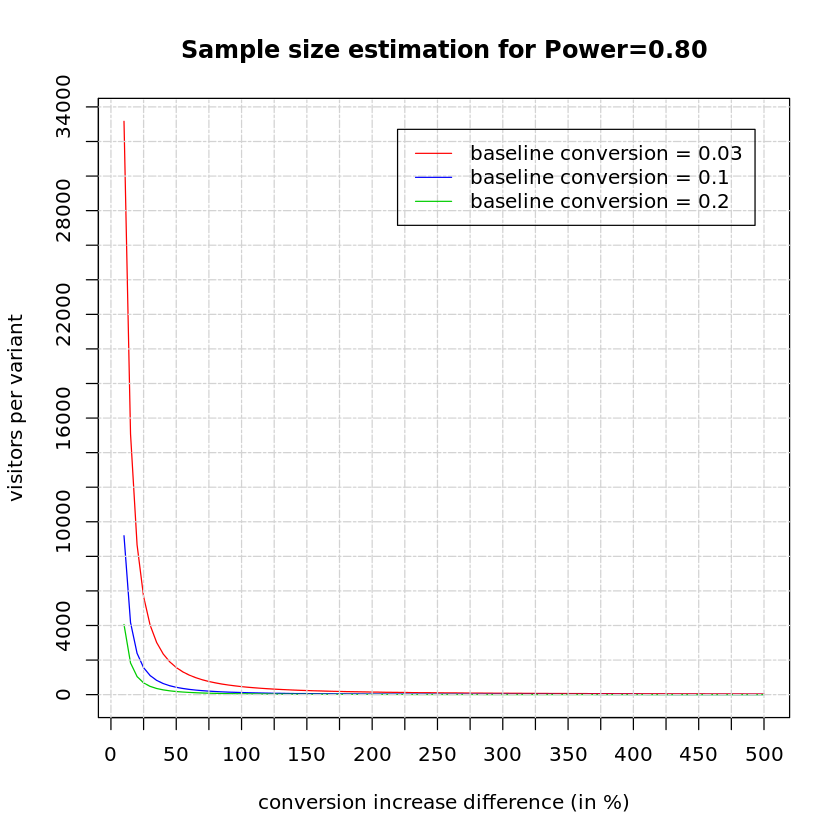
\includegraphics[width=0.8\linewidth]{imgs/samplesizefull.png}
	\caption{Sample Size Calculation}
	\label{fig:samplesize}
\end{figure}
\begin{figure}[ht]
	\centering
	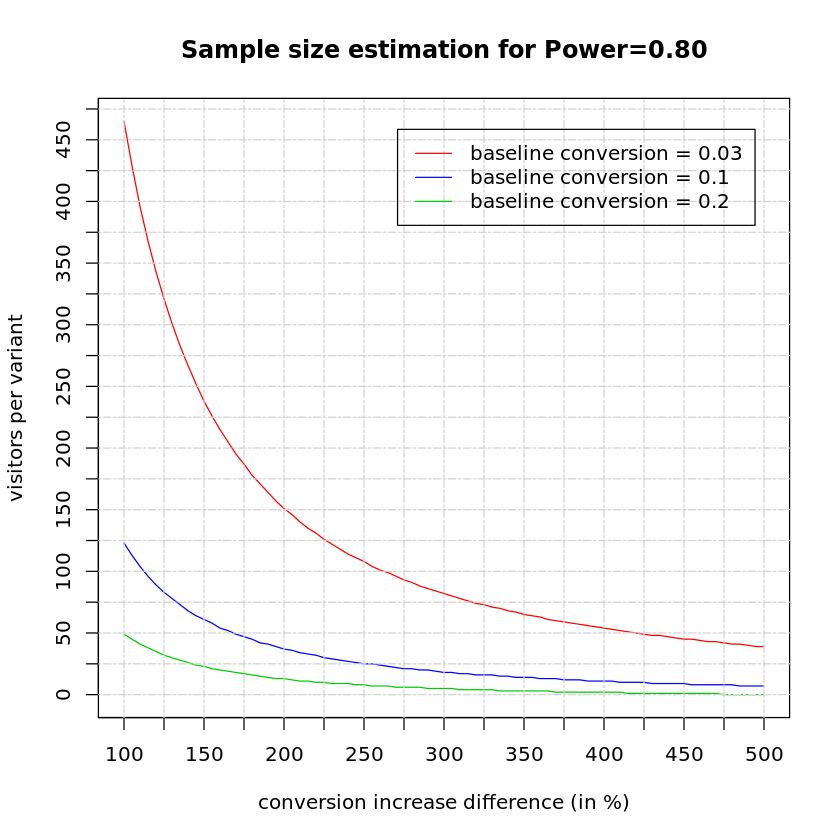
\includegraphics[width=0.8\linewidth]{imgs/samplesize.png}
	\caption{Sample Size Calculation (zoomed in on tail)}
	\label{fig:samplesize2}
\end{figure}
\FloatBarrier

\section{Fluid generations}
In order to speed up the process we will use \textit{fluid generations}. Fluid generations means that the variants of different generations can overlap. For example, some variants from generation 1 and some variants from generation 2 might be evaluated at the same time.\\

Now that we know the relation between the difference of the variants and the number of users needed to find that difference, we can determine how good or how bad a variant is based on how big the difference is. Variants are placed in one of the three categories: worst variants, mediocre variants and best variants.\\

\begin{figure}[ht]
	\centering
	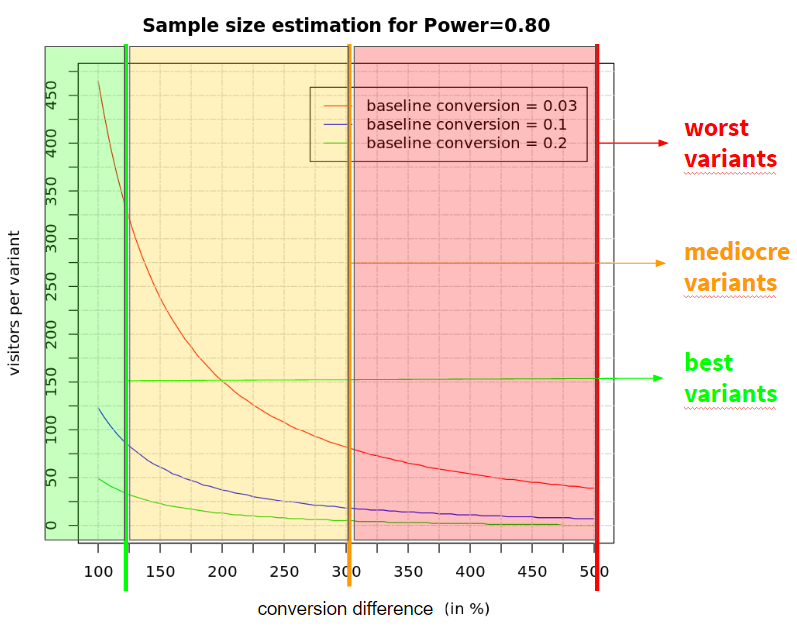
\includegraphics[width=\linewidth]{imgs/treshold_examples.PNG}
	\caption{Threshold Examples}
	\label{fig:te}
\end{figure}
\FloatBarrier
If a significant difference between the worst variant and the best variant is found with only a small amount of visitors for each variant, then we know that the difference has to be big. This is because significant differences with small amount of users are only detectable when they are large. Depending on how many visitors the website has, we can determine thresholds for the amount of visitors for each category. At each threshold level a ANOVA test will be performed.\\

The variants that have significant differences with the best variant that are found in the first threshold (with the least amount of users) are labeled as the worst variants. These worst variants are removed immediately from the population and already replaced with random new variants from the next generation. The variants that have a significant difference with the best variant in the next threshold level are labeled mediocre variants and will be mutated immediately. The remaining variants are labeled as the best variants and they will be combined (crossover) to generate the rest of the variants for the next generation.\\

By replacing variants early on we can already test variants from the next generation, even though the current generation is still being evaluated. This way we have a mix of variants from two different generations to speed up the process. We call this overlapping of variants from different generations fluid generations. An example of the threshold levels used for the fluid generations can be found in Figure~\ref{fig:te}.



\chapter{System Architecture and Implementation}
This section explains the implementation of AMOS into a framework that can be used to easily run a website optimization test. We will also discuss the system architecture and the various design choices.\\

\begin{figure}[ht]
	\centering
	\includegraphics[width=0.9\linewidth]{imgs/flowchart.png}
	\caption{System Architecture Flowchart}
	\label{fig:flowchart}
\end{figure}

Figure~\ref{fig:flowchart} shows the system architecture and the flowchart of the implementation of AMOS into a framework. The website owner starts by filling in the allowed ranges for values for the features to be tested. These settings are then stored on the back-end server and the starting population with variants is created. A tracker is placed on the website which asks the back-end server for a variant before the page is displayed when a user visits the website. The back-end server will give a random variant from the population and the tracker will render this on the website. Then we collect feedback to evaluate the fitness value of the variant. A new population is created when enough users have visited all the variants in the current population.
\begin{enumerate}
	\item \textbf{settings:} Website owner fills in settings about which elements to optimize and what restrictions he wants on those elements on his website.
	\item \textbf{store:} Front-end server stores info in DB on the back-end server and back-end server generates starting \emph{population} for each profile.
	\item \textbf{tracker:} Front-end server generates a tracker that the website owner can include on his website.
	\item \textbf{visit:} User visits a website which has the tracker included with a given \emph{IP address} on time \emph{t}.
	\item \textbf{profile:} Tracker sends time \emph{t} and \emph{IP} to the back-end server page load and the back-end server assigns the user to a certain profile based on at least the time \emph{t} and the \emph{location} of the IP address.
	\item \textbf{variant:} Back-end server returns a variant chosen from the population of that profile. The tracker then injects this variant as CSS to the website before the page is loaded. Once the back-end server has enough information for all the variants in the population to determine a good fitness for each variant, a new population is created from the previous variants (with cross-over, mutation and selection)
	\item \textbf{feedback:} Once the website is loaded, the tracker monitors the action of the visitors and informs the back-end server about the \emph{goals} of the website. For example, these goals can be number of clicks, time on page, conversion, number of sign-ups etc. This information can be used by the \emph{fitness function}. 
\end{enumerate}

\section{PHP front-end Server}
The front-end server is build in PHP. The choice for PHP was simply because it is a simple and accepted language for websites. The front-end server is a simple tool which converts your settings to JSON and talks to the back-end server only once. As PHP has built in tools to convert submitted form info into JSON format, PHP seemed the fastest and most simple choice.
Also, there is some JavaScript used to create the dynamic settings form where users can easily add and remove elements and features. A screenshot of this tool can be found in Figure~\ref{fig:settings} in the next section.

\section{JavaScript Tracker}
The tracker is created with JavaScript. The choice for JavaScript is also an easy one as it is the only fully supported language for dynamic DOM tree changes (changes in the HTML code) in browsers. AJAX calls are used to dynamically talk to the back-end server asynchronously (in the background) to retrieve the correct variant and to give feedback. This way the visitors are not even seeing any communication between the website and our back-end server.

\section{Java back-end Server}
The back-end server needs to be able to respond to requests as quickly as possible, because we do not want to cause too much delay when the visitor of the website has to wait for a variant to be returned. It also needs to be able to handle many and multiple requests at the same time. Therefore, instead of using the more simpler PHP language, we used JAVA to build this server. JAVA has better performance than PHP and it has more native support for multi-threading. Even though this was not yet needed for the scope of this thesis, we wanted to be future-proof and therefore wanted to be as scalable as possible. 
\section{Database}
The Entity-Relation Diagram of the Postgresql database can be found in Figure~\ref{fig:erd}. When a website owner fills in the settings on the front-end server, the back-end server will store those settings in the `website` table. This table contains the website id and url, the settings filled in on the front-end server and the current generation the test on the website is in. The back-end server then stores the individuals (which are created with the settings from the `website` table) in the `individual` table. This table can store individuals for multiple websites by having a link to the `website\_id` and can also have multiple individuals for each user profile. This is useful when you want to optimize a website for multiple user profiles. The `profile` table stores the user profiles. The user profiles are currently only based on location and time of visiting the website.\\

The most complex table is the `individual\_goal` table. This table can be used for fitness values (such as conversion) for each individual and for each session. The sessions can be linked to users by looking at the log file for users. This log file contains the session of the user, its IP-address and the time of visiting. This information can be used to categorize a user under a user profile. The log file of user is not displayed in the database scheme in Figure~\ref{fig:erd}. Besides fitness values for individual sessions, the table `individual\_goal` also stores the average fitness value score for each individual for all sessions combined. \\

\begin{figure}[ht]
	\centering
	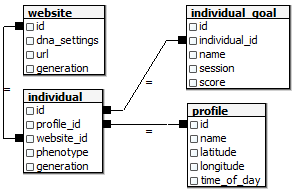
\includegraphics[width=0.6\linewidth]{imgs/erd.PNG}
	\caption{Entity-Relation Diagram from Postgresql Database}
	\label{fig:erd}
\end{figure}
\FloatBarrier

\section{Sessions}
To prevent that visitors get to see a new variant of the website each time they reload the page or navigate to another page within the website, we preserved their sessions in a cookie. A cookie is a small block of data sent from the website to the browser of the user and is stored there. Their session is stored alongside with the id of the variant the user got the first time it visited the site. That same variant is used while their session is valid. Sessions are valid for one day. The sessions ID are stored along the visitors IP and time of visiting in a log file. The same session ID's are also used to store the fitness values for the individuals. This way a single fitness value for an individual can be linked to a user.
\FloatBarrier

\chapter{Evaluation}
With AMOS implemented in a usable framework we can now test if the algorithm can improve the conversion rate and test how many visitors it needs. By looking at the conversion rate we tackle the unrealistic apriori fitness value assumption as discussed in Section~\ref{Theoretical Genetic Algorithm Framework}. We also need to tackle the environment with simulated users. Therefore we will evaluate AMOS on a real live website with real visitors. First the design of the evaluation is explained, then the results of the evaluation are presented and discussed.
\section{Setup}
The design of the evaluation of AMOS is explained in this section. We start by looking at the metrics that need to be evaluated. Next the deployment organisation and the features that will be used for the test are discussed. Finally we clarify the parameters used for the genetic algorithm.

\subsection{Evaluation metrics}
We evaluate the optimization process based on two metrics: \textit{performance} and \textit{efficiency}.
\begin{itemize}
	\item \textbf{Performance}. The performance of the algorithm is the speed of the optimization process. This is measured by looking at the number of visitors needed to see significant changes in the conversion rate. The performance of our algorithm will be compared to more traditional optimization techniques, such as A/B testing and multivariate testing.
	\item \textbf{Efficiency}. The efficiency of the algorithm is how well it will improve the conversion rate for each generation and compare these generations to each other. However, keep in mind that just as with A/B testing and multivariate testing these results are heavily dependent on the type of test you are performing: The bigger the changes are and the more features you adapt, the more chance you have of seeing an increase in the conversion rate.
\end{itemize}

\subsection{Deployment organisation}
Entertainment Agency Evenses~\cite{evenses} was willing to participate in this live experiment. Evenses is a company where you can book all sorts of entertainment for your events. Their website evenses.com has about 10.000 to 15.000 visitors per month. Visitors of their site participated (unknowingly) in the experiment for 1.5 months.

\subsection{Workload and search space}
The website evenses.com has a quotation form were visitors can ask for a price estimation for the entertainment they want to book. The more people fill in and send this form, the more sells Evenses can make. That quotation form is the most important tool of their website as it is their main source of income. We decided to experiment with changing certain features of the button of that form:
\begin{itemize}
	\item \textbf{font-size} - 14px - 25px
	\item \textbf{Text value} - "check beschikbaarheid"\\\tab[1.85cm] - "vrijblijvend aanvragen"\\\tab[1.85cm] - "vrijblijvende offerte"
	\item \textbf{background-color} - fixed color intensity (saturation)\\\tab[3.05cm] - fixed lightness\\\tab[3.05cm] - hue completely free
	\item \textbf{hover-color} - fixed color intensity (saturation)\\\tab[1.97cm] - fixed lightness\\\tab[1.97cm] - hue completely free
\end{itemize}

Given these features with these restrictions we can now calculate how big our search space is:
$$\text{Number of possibilities: } 11*360*360*3 = \textbf{4.276.800 variants}$$

Even though we only change four features and even set restrictions on those features, the search space is still too big to handle using a brute-force approach.\\

These features and the element to which these features need to be applied can be filled in with a tool running on the front-end server. This tool converts the developer settings to proper JSON format and sends it to the backend-server. This tool is shown in Figure~\ref{fig:settings}. The backend-server stores the settings and creates the starting population with random values from the range specified in the JSON. Once that is ready, the backend-server creates a tracker for evenses.com which is returned to the front-end server. That tracker is placed in the source code of evenses.com. When an users visits evenses.com, the tracker will talk to the back-end server before the page loads and retrieves a random variant to be displayed on the website. The tracker will also send the feedback to the back-end server


\begin{figure}[ht]
	\centering
	\hspace*{-1.7cm}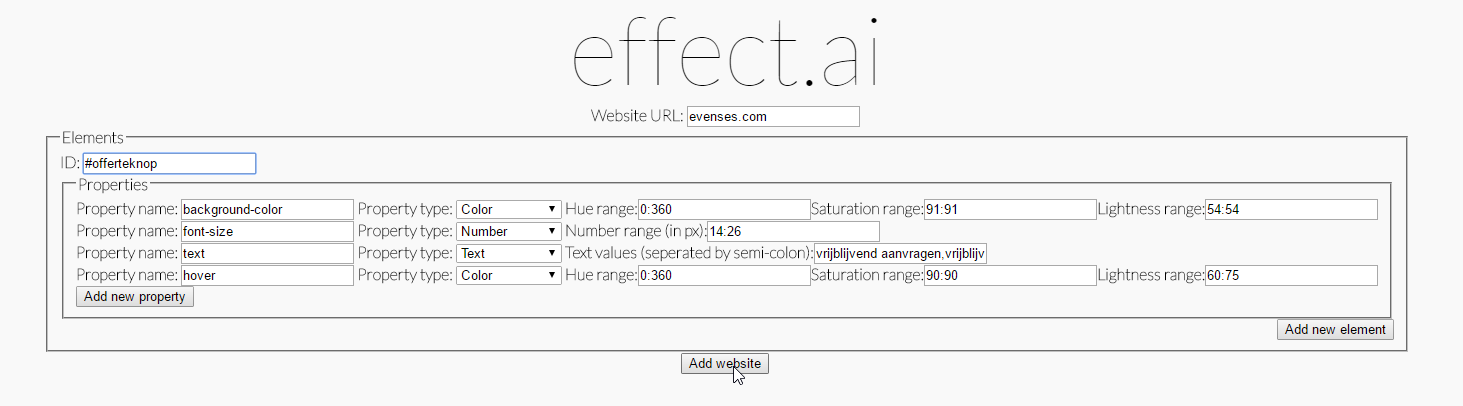
\includegraphics[width=1.3\linewidth]{imgs/settings.png}
	\caption{Tool to input the settings for the test for a website and retrieve a tracker.}
	\label{fig:settings}
\end{figure}

\subsection{GA parameters}
The parameter values used for the evaluation test are displayed in Table~\ref{tab:par}.
As we only had a short time-span to test this on evenses.com and the website has about 10.000 visitors per month, we kept the population size small, so that we could still have multiple generations for this test. However, for bigger website with more visitors a bigger population size might improve the results.\\

As we wanted to at least have a few generations completed within this short time-span, we used threshold values for the number of visitors needed in such a way that the algorithm would still find significant differences between the variants, but also moves on quickly to the next generation. Therefore, small differences are unlikely to be detected with these settings. If the test was run for a longer period of time, the threshold values for the number of visitors needed can be set to higher values to also detect smaller differences. To speed up the process of moving on to the next generation, we used an alpha value of 0.90 instead of the more usual 0.95. The alpha value to compare different variants from all generations at the end of the test is still 0.95.\\

The test has run for approximately one month and we managed to complete 3 generations (whilst the 4th generation is still running). Note that most genetic algorithms have parameter values for selection, mutation and crossover. However, our algorithm uses fluid generation and threshold values for the number of visitors needed to determine these parameters values. See Section~\ref{Fluid generations} for more details on fluid generations.

\begin{table}[h]
	\centering
	\begin{tabular}{|l|l|}
		\hline
		\textbf{Parameter}                    & \textbf{Value}           \\ \hline
		Population Size                       & 10 variants              \\ \hline
		\(\alpha\) for moving to next gen     & 0.1 (90\% significance)  \\ \hline
		\(\alpha\) for comparing all variants & 0.05 (95\% significance) \\ \hline
		\(\beta\) for sample size calculation & 0.2 (power value = 0.8)  \\ \hline
		Threshold value (worst variants)      & 150 visitors per variant \\ \hline
		Threshold value (mediocre variants)   & 300 visitors per variant \\ \hline
	\end{tabular}
	\caption {Parameter values for AMOS}
	
	\label{tab:par}
\end{table}

\section{Results}
First, this section presents and discusses the results of the live test on evenses.com. Then we will test the two evaluation metrics \textit{performance} and \textit{efficiency} based on these results.\\

Figure~\ref{fig:gen1} shows the initial population used in our experiment. According to section~\ref{Genetic Algorithm}, the ten different variants of the initial population were randomly selected from the search space with values within the range we specified. The submission form has various colors and the submit button on the form has various font-sizes and text values. What the figures do not show is the background color of the button on mouse-over.\\

\begin{figure}[ht]
	\hspace*{-1.6cm}\subfloat[Gen 1: 1]{
\includegraphics[width = 1.3in,valign=t]{imgs/gen1/evenses_knop1.PNG}} 
	\subfloat[Gen 1: 2]{
\includegraphics[width = 1.3in,valign=t]{imgs/gen1/evenses_knop2.PNG}} 
	\subfloat[Gen 1: 3]{
\includegraphics[width = 1.3in,valign=t]{imgs/gen1/evenses_knop3.PNG}} 
	\subfloat[Gen 1: 4]{
\includegraphics[width = 1.3in,valign=t]{imgs/gen1/evenses_knop4.PNG}} 
	\subfloat[Gen 1: 5]{
\includegraphics[width = 1.3in,valign=t]{imgs/gen1/evenses_knop5.PNG}} \\
	\hspace*{-1.6cm}\subfloat[Gen 1: 6]{
\includegraphics[width = 1.3in,valign=t]{imgs/gen1/evenses_knop6.PNG}} 
	\subfloat[Gen 1: 7]{
\includegraphics[width = 1.3in,valign=t]{imgs/gen1/evenses_knop7.PNG}} 
	\subfloat[Gen 1: 8]{
\includegraphics[width = 1.3in,valign=t]{imgs/gen1/evenses_knop8.PNG}} 
	\subfloat[Gen 1: 9]{
\includegraphics[width = 1.3in,valign=t]{imgs/gen1/evenses_knop9.PNG}} 
	\subfloat[Gen 1: 10]{
\includegraphics[width = 1.3in,valign=t]{imgs/gen1/evenses_knop10.PNG}}
	
	\caption{Variants from generation 1}
	\label{fig:gen1}
\end{figure}
\FloatBarrier
When all the variants had enough visitors to calculate the conversion rate reliably (see Section~\ref{Amount of visitors needed: sample size calculation}), the genetic algorithm creates a second generation. Figure~\ref{fig:gen2} shows the second generation. We can notice that the lighter colors, such as green and yellow, are already filtered out from the population. This is because they had the lowest conversion rates and that might be due to the fact that the white text becomes harder to read~\cite{leavitt2006research, thatcher2002constructing}. We can also see that 7 out of the 10 variants have as button text "Check Beschikbaarheid". This is the most non-committal text and that is probably why this text value performs better than the other two~\cite{cta}.\\

\begin{figure}[ht]
	\hspace*{-1.6cm}\subfloat[Gen 2: 1]{
\includegraphics[width = 1.3in,valign=t]{imgs/gen2/evenses_gen2_1.PNG}} 
	\subfloat[Gen 2: 2]{
\includegraphics[width = 1.3in,valign=t]{imgs/gen2/evenses_gen2_2.PNG}} 
	\subfloat[Gen 2: 3]{
\includegraphics[width = 1.3in,valign=t]{imgs/gen2/evenses_gen2_3.PNG}} 
	\subfloat[Gen 2: 4]{
\includegraphics[width = 1.3in,valign=t]{imgs/gen2/evenses_gen2_4.PNG}} 
	\subfloat[Gen 2: 5]{
\includegraphics[width = 1.3in,valign=t]{imgs/gen2/evenses_gen2_5.PNG}} \\
	\hspace*{-1.6cm}\subfloat[Gen 2: 6]{
\includegraphics[width = 1.3in,valign=t]{imgs/gen2/evenses_gen2_6.PNG}} 
	\subfloat[Gen 2: 7]{
\includegraphics[width = 1.3in,valign=t]{imgs/gen2/evenses_gen2_7.PNG}} 
	\subfloat[Gen 2: 8]{
\includegraphics[width = 1.3in,valign=t]{imgs/gen2/evenses_gen2_8.PNG}} 
	\subfloat[Gen 2: 9]{
\includegraphics[width = 1.3in,valign=t]{imgs/gen2/evenses_gen2_9.PNG}} 
	\subfloat[Gen 2: 10]{
\includegraphics[width = 1.3in,valign=t]{imgs/gen2/evenses_gen2_10.PNG}}
	
	\caption{Variants from generation 2}
	\label{fig:gen2}
\end{figure}
\FloatBarrier

Figure~\ref{fig:gen3} shows the third generation of our experiment. We see fewer differences between this generation and the second one than between the second and the first. This may be explained by the fact that the first generation was completely random, while the second generation already incorporates information about the end goal. Namely, the second generation was generated with the best variants from the first generation.\\

In the third generation we see that 9 out of the 10 variants have as text value "Check Beschikbaarheid", so this seems to be the best value for the text feature. We also see that the red, orange and blue colors are performing well (as they are both still present in this generation in great numbers). This might be due to different preferences of the visitors of the website.\\

In an ideal world, we want to give each user their own optimized variant. In Section~\ref{Future work} we will explain how these different user preferences might be grouped together in \textit{user profiles}. By having multiple user profiles each profile would get their own optimized variant. If we look at this test as an example, there might be two different User Profiles: one that gets to see the orange/red button and the other one that gets to see the blue button. However, before we are allowed to do this, we need to find a relation between one or multiple attributes of the visitors and the preferred color of the form.\\

\begin{figure}[ht]
	\hspace*{-1.6cm}\subfloat[Gen 3: 1]{
\includegraphics[width = 1.3in,valign=t]{imgs/gen3/evenses_gen3_1.PNG}} 
	\subfloat[Gen 3: 2]{
\includegraphics[width = 1.3in,valign=t]{imgs/gen3/evenses_gen3_8.PNG}} 
	\subfloat[Gen 3: 3]{
\includegraphics[width = 1.3in,valign=t]{imgs/gen3/evenses_gen3-9.PNG}} 
	\subfloat[Gen 3: 4]{
\includegraphics[width = 1.3in,valign=t]{imgs/gen3/evenses_gen3_4.PNG}} 
	\subfloat[Gen 3: 5]{
\includegraphics[width = 1.3in,valign=t]{imgs/gen3/evenses_gen3_2.PNG}} \\
	\hspace*{-1.6cm}\subfloat[Gen 3: 6]{
\includegraphics[width = 1.3in,valign=t]{imgs/gen3/evenses_gen3_6.PNG}} 
	\subfloat[Gen 3: 7]{
\includegraphics[width = 1.3in,valign=t]{imgs/gen3/evenses_gen3_7.PNG}} 
	\subfloat[Gen 3: 8]{
\includegraphics[width = 1.3in,valign=t]{imgs/gen3/evenses_gen3_5.PNG}} 
	\subfloat[Gen 3: 9]{
\includegraphics[width = 1.3in,valign=t]{imgs/gen3/evenses_gen3_3.PNG}} 
	\subfloat[Gen 3: 10]{
\includegraphics[width = 1.3in,valign=t]{imgs/gen3/evenses_gen3_0.PNG}}
	
	\caption{Variants from generation 3}
	\label{fig:gen3}
\end{figure}
\FloatBarrier

\subsection{Efficiency}
To test whether the genetic algorithm can improve web design, we need to check the average values of each generation and compare them with each other to see if there is a significant improvement. Figure~\ref{fig:comparegen} shows all the conversion rates of each variant. The red circles are from the first generation, the blue from the second and the green from the last. The three lines indicate the averages of the conversion rates for each generation. Table \ref{tab:infogen} shows the variant with the lowest conversion rate, the variant with the highest conversion rate and the average conversion rate for each generation.\\

\begin{figure}[ht]
	\centering
	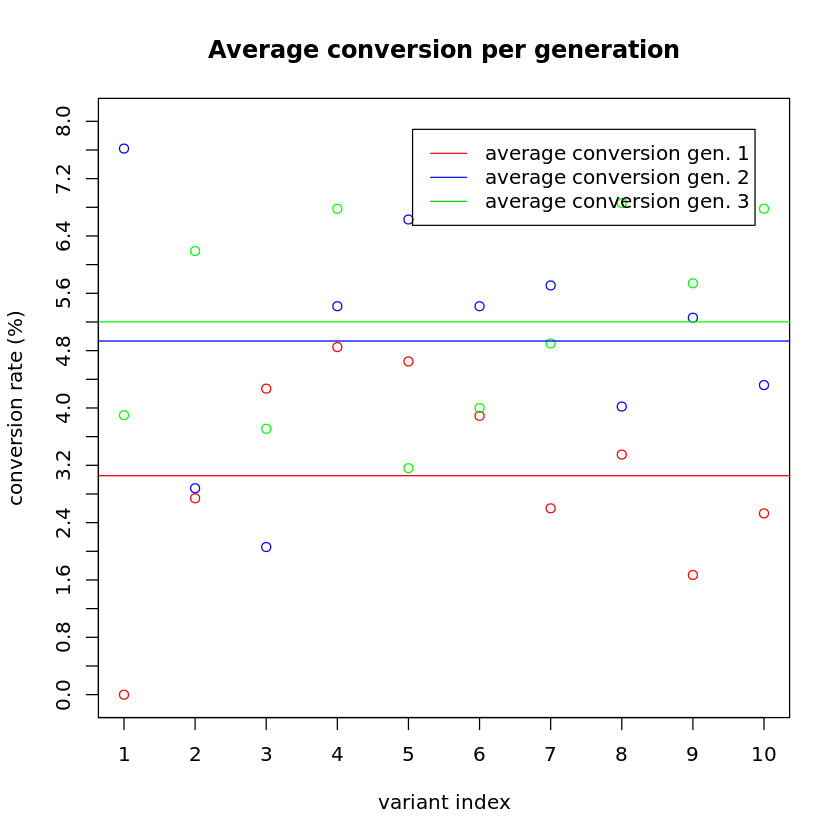
\includegraphics[width=0.8\linewidth]{imgs/comparegen.png}
	\caption{Compare conversion of different generations}
	\label{fig:comparegen}
\end{figure}
\FloatBarrier
\begin{table}[h]
 \begin{tabular}{|p{2cm}|p{3.5cm}|p{3.5cm}|p{3.5cm}|}
    \hline
\textbf{Generation} & \textbf{Lowest conversion} & \textbf{Highest conversion} & \textbf{Average conversion} \\ \hline
    1          & 0                 & 4.85               & 3.055                                                     \\\hline
    2          & 2.06              & 7.62               & 4.934                                                     \\\hline
    3          & 3.16              & 6.86               & 5.202                                                     \\\hline

	\end{tabular}
	\caption {Statistics for each generation}
	
	\label{tab:infogen}
\end{table}

We can already see that each new generation produces a better average conversion rate. In order to check whether these differences are significant, we will use the two-sample z-test to compare the sample proportions. The following formula is used to calculate the z-score~\cite{brown2001interval}:

$$Z=\dfrac{(\hat{p}_1-\hat{p}_2)}{\sqrt{\dfrac{\hat{p}_1(1-\hat{p}_1)}{n_1}+\dfrac{\hat{p}_2(1-\hat{p}_2)}{n_2}}}$$\\

Applying this formula to generations 1 and 2 gives us:

$$\text{z-score} = -3.0337942$$
$$\text{two-tailed p-value} = 0.001207$$

With this p-value we can reject the null hypothesis stating that the two conversion rates are the same. Therefore, the difference between the conversion rates of generation 1 and 2 is significant. \\

If we apply the formula to generation 2 and 3, we obtain:
$$\text{z-score} = -0.40379783$$
$$\text{two-tailed p-value} = 0.343180696$$

With this p-value we can \textit{not} reject the null hypothesis stating that the two conversion rates are the same. Therefore, the difference between the conversion rate of generation 2 and 3 is not significant.\\

Even though the increase in conversion rate is not significant yet, Table \ref{tab:infogen} shows that the lowest variant from the second generation has a significantly lower conversion rate than the lowest variant from the third generation. Therefore we can still conclude that generation 3 is an improvement over generation 2, because generation 3 contains less 'bad' variants. Table \ref{tab:comgen} shows a summary of the statistics used for the comparison of the different generations.\\

\begin{table}[h]
 \begin{tabular}{|p{2cm}|p{3.5cm}|p{3.5cm}|p{3.5cm}|}
    \hline
\textbf{Generation} & Compare to \newline previous generation \newline \textbf{Z-value} & Compare to \newline previous generation \newline \textbf{P-value} & Compare to \newline previous generation \newline \textbf{Significant} \\ \hline
    1                       & -                                       & -                                       & -                                           \\\hline
    2                       & -3.0337942                              & 0.001207                                & Yes                                         \\\hline
    3                       & -0.40379783                             & 0.343180696                             & No                                          \\\hline

	\end{tabular}
	\caption {Compare different generations}
	\label{tab:comgen}
\end{table}

\FloatBarrier
\subsection{Performance}
Another important aspect is performance. Here, we take a look at the number of visitors that was needed to run this experiment (GA) compared to the traditional website optimizing techniques: A/B testing (AB) and multivariate testing (MV). We assume that the same variants that were tested using our genetic algorithm are also going to be tested with the AB and MV approaches.\\

Note however that the outcome of this comparison is dependent on the variants that are being tested. We are only comparing the methods of the different optimization techniques, not the quality of the approaches. The quality of the three different approaches is very hard to compare to each other, as the quality of the test depends on which variants the designer picks. It would be very unlikely that the same variants are picked as the automatically generated variants from the genetic algorithm. By assuming that the quality is the same for all three approaches (by using the same variants) gives us insight into the number of visitors required by the three different optimization techniques. \\

Figure~\ref{fig:comparesota} shows the estimated number of visitors needed for each optimization technique to test the 30 variants that were tested with our genetic algorithm. To test these 30 variants with A/B testing you would need at least 15 A/B test. You would need one big or multiple smaller tests to test these 30 variants with multivariate testing. The estimations are calculated with the formulas from the \textit{Sample Size Calculation} section earlier on in this thesis. We see here that the 15 A/B tests would take the most visitors (and thus time) to complete. The multivariate testing is second best and our genetic algorithm approach needs the least visitors and is therefore the fastest in this example.\\

\begin{figure}[ht]
	\centering
	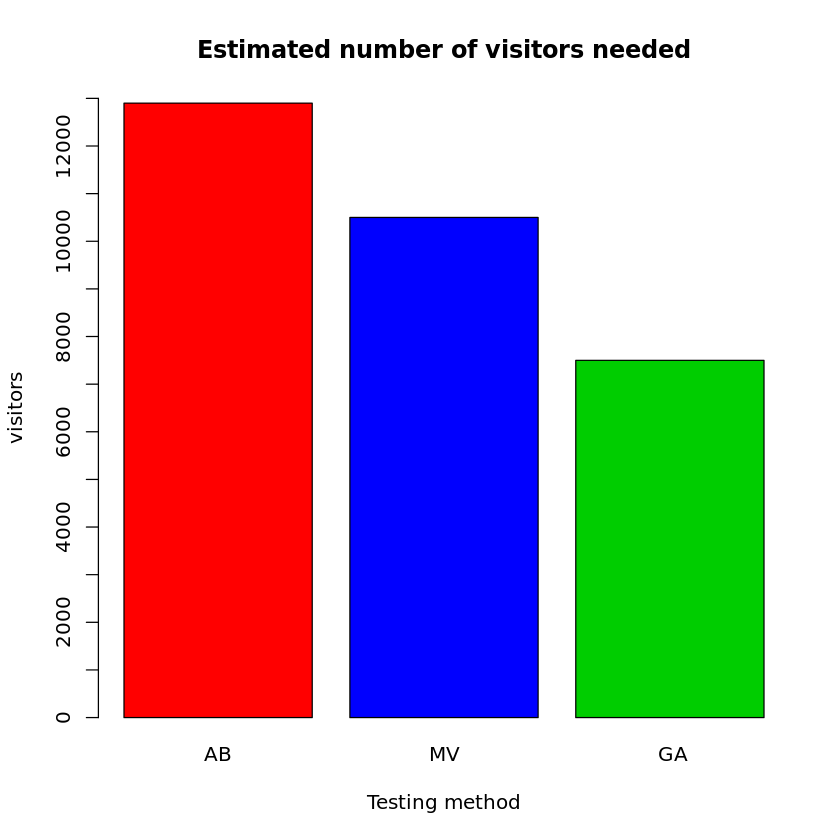
\includegraphics[width=0.8\linewidth]{imgs/comparesota.png}
	\caption{Compare different optimization techniques}
	\label{fig:comparesota}
\end{figure}
\FloatBarrier

The difference between A/B testing and multivariate testing can be explained because the results of the A/B test are calculated with a simple Student's t-test and the results from the multivariate test are calculated with ANOVA. ANOVA has a better power than multiple t-test~\cite{miller2013analysis} and needs therefore less visitors. Multivariate testing and genetic algorithm approach both use ANOVA for their statistical calculations. The difference between multivariate testing and genetic algorithm is due to the fact that we use fluid generations in our genetic algorithm. Note that if such a technique would be used for multivariate testing, the amount of visitors needed for multivariate testing and genetic algorithm would be the same.



\chapter{Conclusions}
Current techniques used for website optimization, such as A/B testing and multivariate testing, where different variants of the website are compared to each other, suffer from several limitations. The sampling of variants from the search space is a time-consuming manual task that requires domain knowledge. Also, the quality of the interpretation of the statistics of the test affects  the quality of variants created for the next test. Due to these limitations we investigated in this thesis whether genetic algorithms could \textit{automate} and \texit{improve} the real-world optimization process of web design. After accurately identifying the problems with the traditional optimization techniques, we formalized website optimization as a search problem. By doing this, we were able to create an algorithm based on a combination of hill climbing and genetic algorithms with fluid generations to automatically optimize websites. \\

We implemented AMOS in a usable framework to be able to test the algorithm on a live website with real users. The live experiment that was run on the website evenses.com showed that AMOS can indeed be used to automate and improve the website optimization process. The two evaluation metrics \texit{effectiveness} and \texit{performance} were used to validate AMOS. The performance, the speed of the optimization process, is measured by looking at the number of visitors needed to see significant changes in the conversion rate. The efficiency of the algorithm is measured by looking at the conversion rates for each generation and see how much it improves. We also compared AMOS to the traditional website optimization techniques.\\

The results of the test show that genetic algorithms can indeed improve the conversion rate automatically without the need of sampling the variants manually. So far, each new generation showed an improvement in conversion rate compared to the previous generation. However, keep in mind that just as with A/B testing and multivariate testing these results are heavily dependent on the type of test you are performing: The bigger the changes are and the more features you adapt, the more chance you have of seeing an increase in the conversion rate.\\

It is hard to compare our algorithm with traditional optimization techniques, because the results are very dependent on the type of test you perform and which variants the designer (or the genetic algorithm) picks. However, The results of the test show that AMOS needs less visitors for testing a few generations of variants than the multiple A/B tests or multivariate tests that would be needed to test the same number of variants. This advantage is due to the fluid generations. AMOS will only work for website optimizing when enough variants are being tested, because it needs to be able to make multiple generations. When a website only needs to test a few variants, it is better to use traditional optimization techniques. We also saw from the live test that every generation improved the average conversion rate so far. This might not be the case when many generations are created, as the changes in the features will become smaller and therefore it will be harder to detect significant changes in the conversion rates.\\

The live experiment we did to test AMOS for website optimization already showed great results and is a strong indicator that genetic algortihms are indeed very useful to automate and improve the website optimization process.\\


\section{Future work}
Although the first evaluation test of AMOS already shows promising results, it still needs to be tested from different perspectives. Tests should be run on different websites and with various different features to be optimized. Also, different parameter settings should be tested in order to refine AMOS. The mutation rate and crossover rate can be adapted as well as the threshold values for the fluid generations. Multiple generation should be used in these tests to see how long the algorithm will continue to improve the conversion rate (or any other business goals).\\

Also, more comparisons between the traditional optimization techniques and AMOS are necessary. Of course, AMOS is a worthy replacement, only if we can show that it is better than traditional optimization techniques.\\

A feature that might make AMOS even more effective and distinctive is the partition of different \textit{user profiles}. Different visitors of the website might have different user preferences. If we can group the users with roughly the same preferences, then each user profile can get their own optimized variant of the website. The grouping of users in user profiles can be based on time, location, gender, age etc. The values easiest to obtain are location (from the IP-address of the user) and the time of visiting. If there is a relation between certain values for features and for example the location of the user or the time of visiting, we can use that relation to create multiple user profiles. For example, users might like darker colors better at night and lighter colors better during daytime. Also, users from different countries might have different preferences.\\

These relations for the user profiles can be detected with machine learning, a technique specialised in pattern recognition~\cite{michalski2013machine}. Next on our roadmap is to check whether this kind of relations exists for the data we obtained during our live test on evenses.com. Critical issues related to this feature would be: analyzing the feasibility of detecting different user profiles; systematic estimation of the number of visitors required to find such relations; study the re-usability of visitor profiles across different websites.
 
\renewcommand\chapter{\origchapter}    

\noindent 
\nocite{*}
\bibliographystyle{IEEEtran}
\bibliography{references}

\begin{appendices}
\chapter{Sample Size Calculation in R} \label{app:R}
\begin{lstlisting}[language=R, caption=Sample Size Calculation in R, label=lst:R]
# parameters
tau=9 # number of comparisons to be made (bonferri correction)
alpha=0.1 # significance level
beta=0.20 # power value
tailed = 2 #two-tailed or one-tailed test
pA=0.03 # baseline conversion
seq_pB = seq(0.1, 5, 0.05) # percentage increase of baseline 

# calculate all sample sizes 
data = NULL
index = 1
for (i in seq_pB) {
    pB=pA+pA*i
    (n=(pA*(1-pA)+pB*(1-pB))*((qnorm(1-alpha/tailed/tau)+qnorm(1-beta))/(pA-pB))^2)
    data[index] = ceiling(n/2)
    index = index+1;
}

# display in graph 
matplot(seq_pB*100, data, type='l', col=c(2,4,3), lty=c(1,1,1), ylab="visitors per variant", xlab="conversion increase difference (in %)", main="Sample size estimation for Power=0.80")
\end{lstlisting}
\end{appendices}





\end{document}
